\documentclass[a4paper,12pt]{article}


\usepackage{minted}
\usepackage[cm]{fullpage}
%\usepackage[a4paper,margin=1in]{geometry}
\usepackage{graphicx}
\usepackage{amsmath}
\usepackage{capt-of}

\setminted[C]{fontsize=\small, tabsize=4, breaklines, linenos}
\setminted[Python]{fontsize=\small, tabsize=4, breaklines, linenos}
\setminted[Ruby]{fontsize=\small, tabsize=4, breaklines, linenos}
\setminted[text]{fontsize=\small, tabsize=4, breaklines, linenos}

%\setlength\parindent{0pt}

\title{Assignment 2 Report}
\author{Julius Putra Tanu Setiaji (A0149787E), Chen Shaowei (A0110560Y)}
\date{19 November 2018}

\begin{document}
\maketitle

\section{Program Design}
The program is implemented in CUDA. The goal is to achieve the best possible speedup. Primary design considerations are:
\begin{itemize}
  \item Ensure maximum utilisation of computation resources.
  \item Minimise overhead as much as possible (especially by reducing the number of branching to prevent idle threads in an SIMT execution model).
  \item Ensure correctness of output by ensuring that only one process writes to result buffer.
\end{itemize}

\section{Program Overview}
\begin{enumerate}
  \item \textit{In host:} Read input.
  \item \textit{In host:} Setup:
  \begin{itemize}
    \item Copy timestamp used to compute hash from host to device.
    \item Copy target value from host to device.
    \item Copy previous hash from host to device.
  \end{itemize}
  \item \textit{In host:} Execute the kernel with the specified blocks-per-grid and threads-per-block.
  \item \textit{In kernel:} Compute initial nonce by calculating $blockId \times threadsPerBlock + threadId$.
  \item \textit{In kernel:} Construct SHA256 input and compute hash.
  \item \textit{In kernel:} Compare first 64 bits of digest with target value.
  \begin{itemize}
    \item If the computed hash is satisfactory, execute an \mintinline{C}{atomicExch((int*)&is_found, 1)} to determine if current thread should write to output buffer.
    \item Otherwise, increment the nonce by the value of $blocksPerGrid \times threadsPerBlock$.
  \end{itemize}
  \item \textit{In kernel:} Check if \mintinline{C}{is_found} is set.
  \begin{itemize}
    \item If set, return.
    \item If unset, go to 5.
  \end{itemize}
  \item \textit{In host:} Wait for kernel to complete by calling \mintinline{C}{cudaDeviceSynchronize()}.
  \item \textit{In host:} Print output.


\end{enumerate}

\section{Points to Note / Implementation Details}
\begin{itemize}
	\item Memory transfer between host and device memory is expensive and should be minimised. In our program, the only memory transfer between host and device are:
  \begin{itemize}
    \item Copying of input and initial parameters from host to device in the setup stage.
    \item Retrieve output value from device to host.
    \begin{itemize}
      \item \textbf{Note:} This is an implicit transfer. The buffer for storing output values is allocated as Unified Memory.
    \end{itemize}
  \end{itemize}
  \item Input values (timestamp, target, previous hash) are stored in constant memory since they are only read, not written to.
  \item A test and set operation \mintinline{C}{atomicExch} is used when a valid nonce is found to ensure that only one thread writes to output buffer.
  \item The completion flag must be marked as \mintinline{C}{volatile} to ensure that Unified Memory optimisations do not cause the variable to be migrated into register/shared/local memory and its value is read from the global memory each time.
  \item Due to the avalanche effect in SHA256, the program searches for valid nonces incrementally starting from 0 for simplicity.
\end{itemize}

\section{Performance Analysis and Discussion}

\subsection{Platform Overview}

Various tests were run on the SoC compute cluster(XGPC) and the Jetson TX2 module in the lab. Given below is an overview of the two platforms:

\begin{itemize}
  \item \textbf{XGPC}
  \begin{itemize}
    \item CPU: $2 \times$ Intel Xeon 4108 (Dual socket)
    \begin{itemize}
      \item 8 Cores
      \item 16 Threads
    \end{itemize}
    \item GPU: NVIDIA Tesla V100-PCIE
    \begin{itemize}
      \item 80 Volta SM
      \item 64 CUDA cores per SM
    \end{itemize}
  \end{itemize}
  \item \textbf{Jetson TX2}
  \begin{itemize}
    \item CPU: NVIDIA Denver2 + ARM Cortex A-57
    \begin{itemize}
      \item 2 + 4 Cores (Heterogeneous)
    \end{itemize}
    \item GPU: NVIDIA
    \begin{itemize}
      \item 2 Pascal SM
      \item 128 CUDA cores per SM
    \end{itemize}
    \item \textit{Note:} System memory is shared between CPU and GPU
  \end{itemize}
\end{itemize}

\section{Kernel Performance}

In this section, we shall discuss the performance of the CUDA kernel. All values reported are 10-run averages. Target exponent of $2^{48}$ is used so as to not overflow the hardware counters when running \texttt{nvprof}.\\
\\
\textit{Note:} The following analysis does not consider the fixed overhead of copying input parameters from host to device and subsequent retrieval of result value. This is discussed in the next section.

\subsection{Kernel Performance on Jetson TX2}

The program was run on the Jetson TX2 with blocks-per-grid values between 1 and 64 and threads-per-block values between 1 and 256.

\begin{center}
  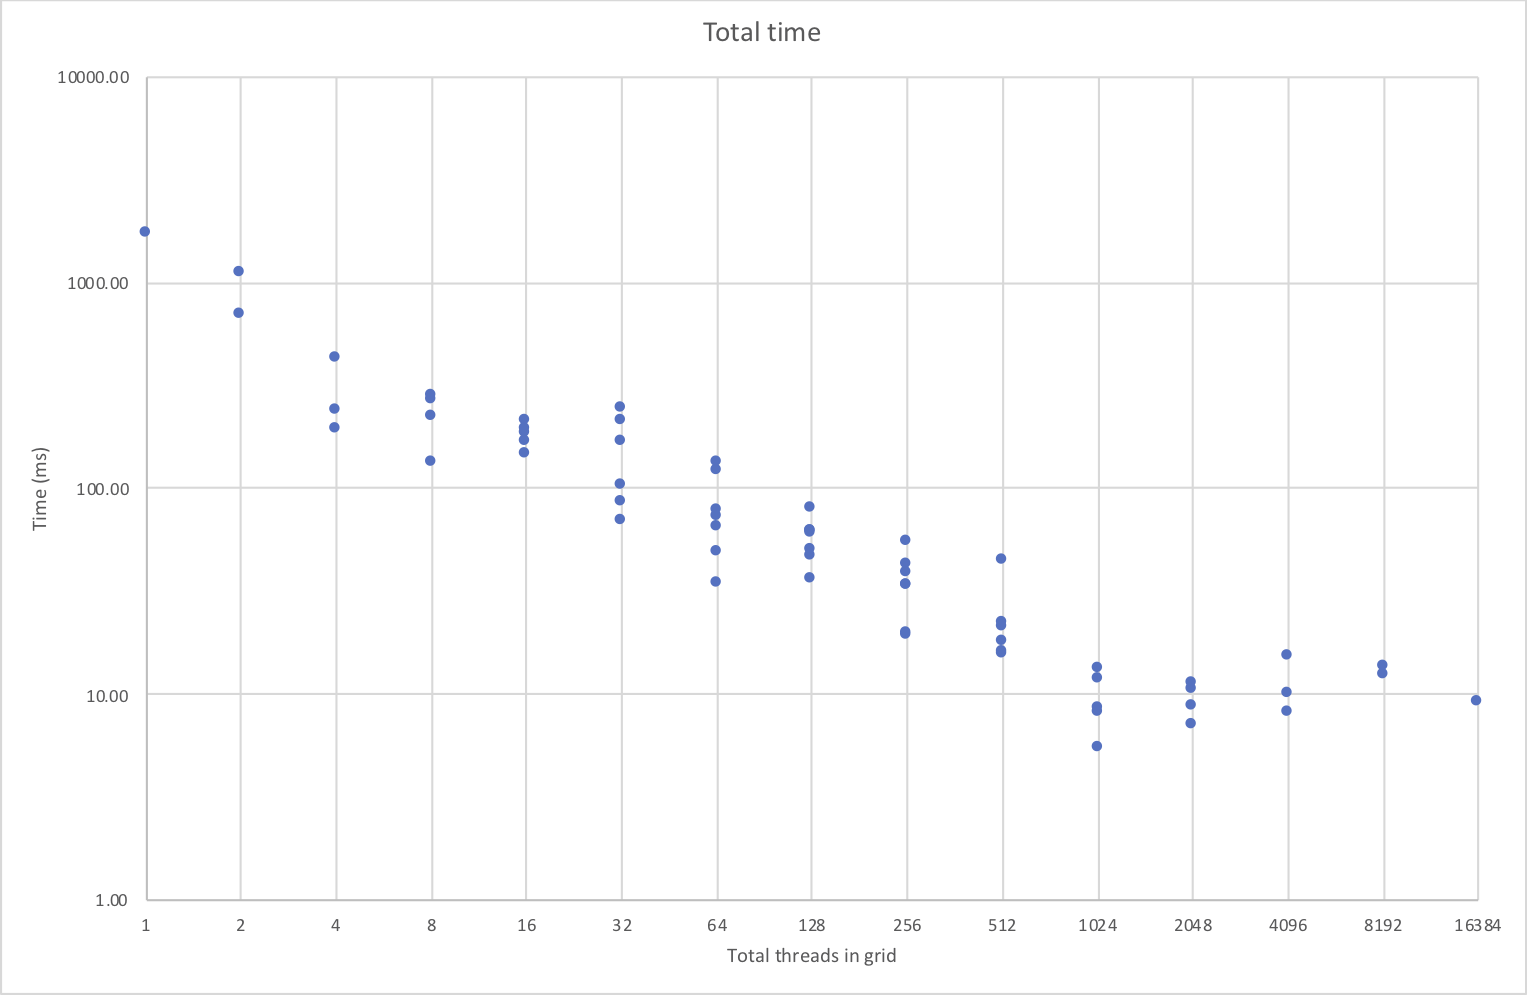
\includegraphics[width=\linewidth]{jetson-time}
  \captionof{figure}{Scatter graph of time taken on Jetson against total threads in grid}
\end{center}

\begin{center}
  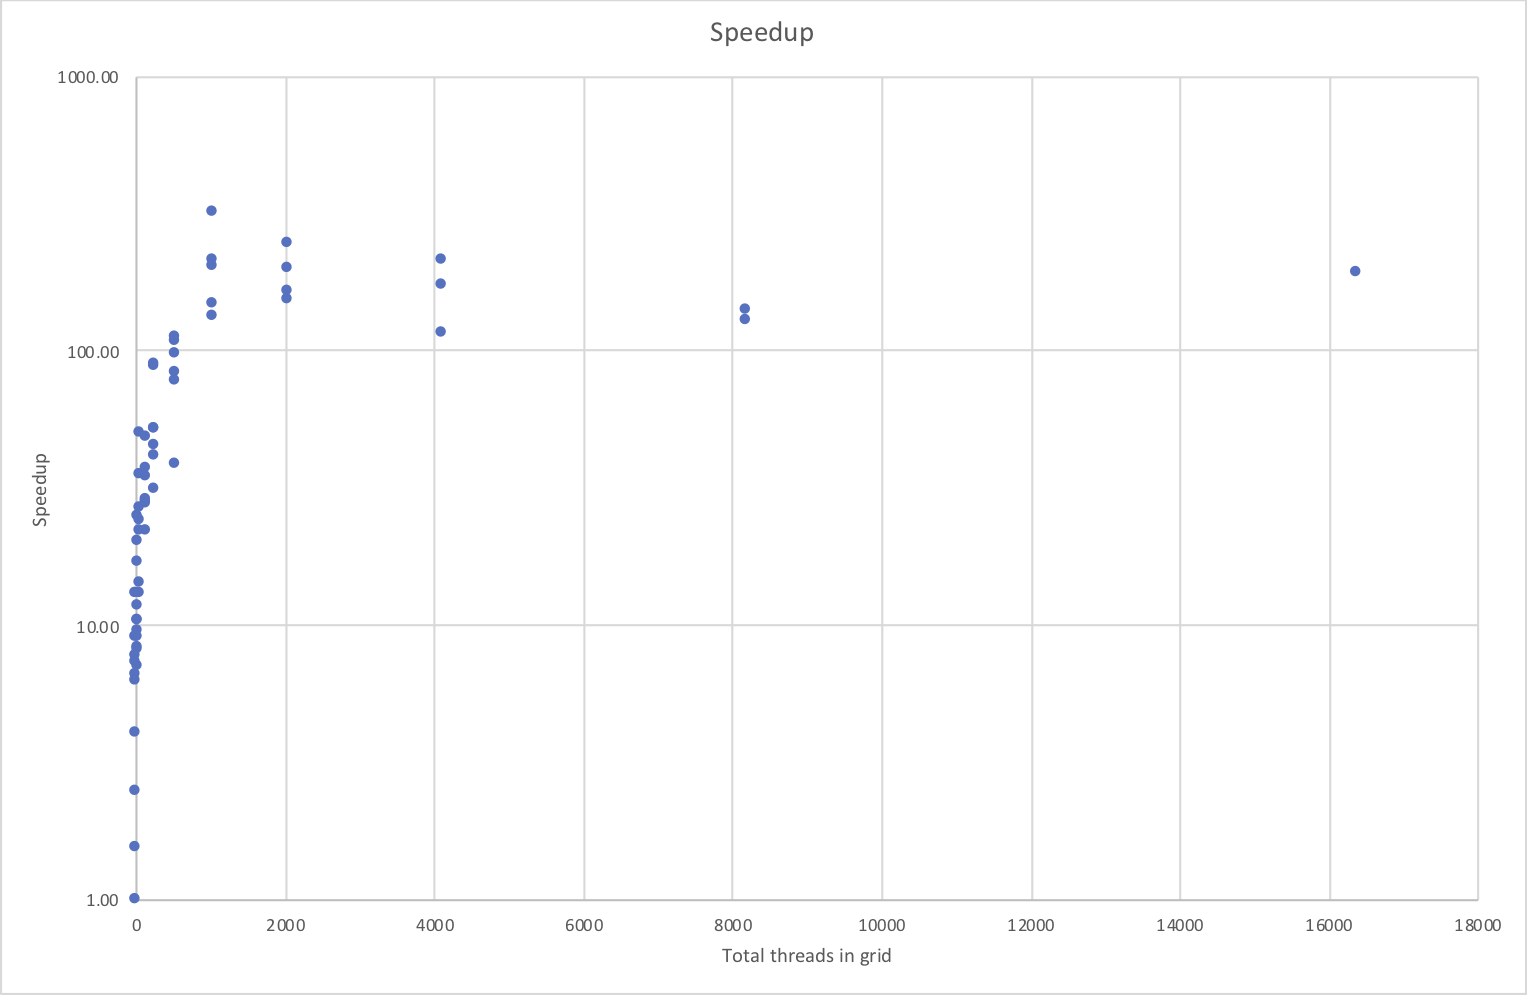
\includegraphics[width=\linewidth]{jetson-speedup}
  \captionof{figure}{Scatter graph of speedup achieved on Jetson as number of threads increases}
\end{center}

\begin{center}
  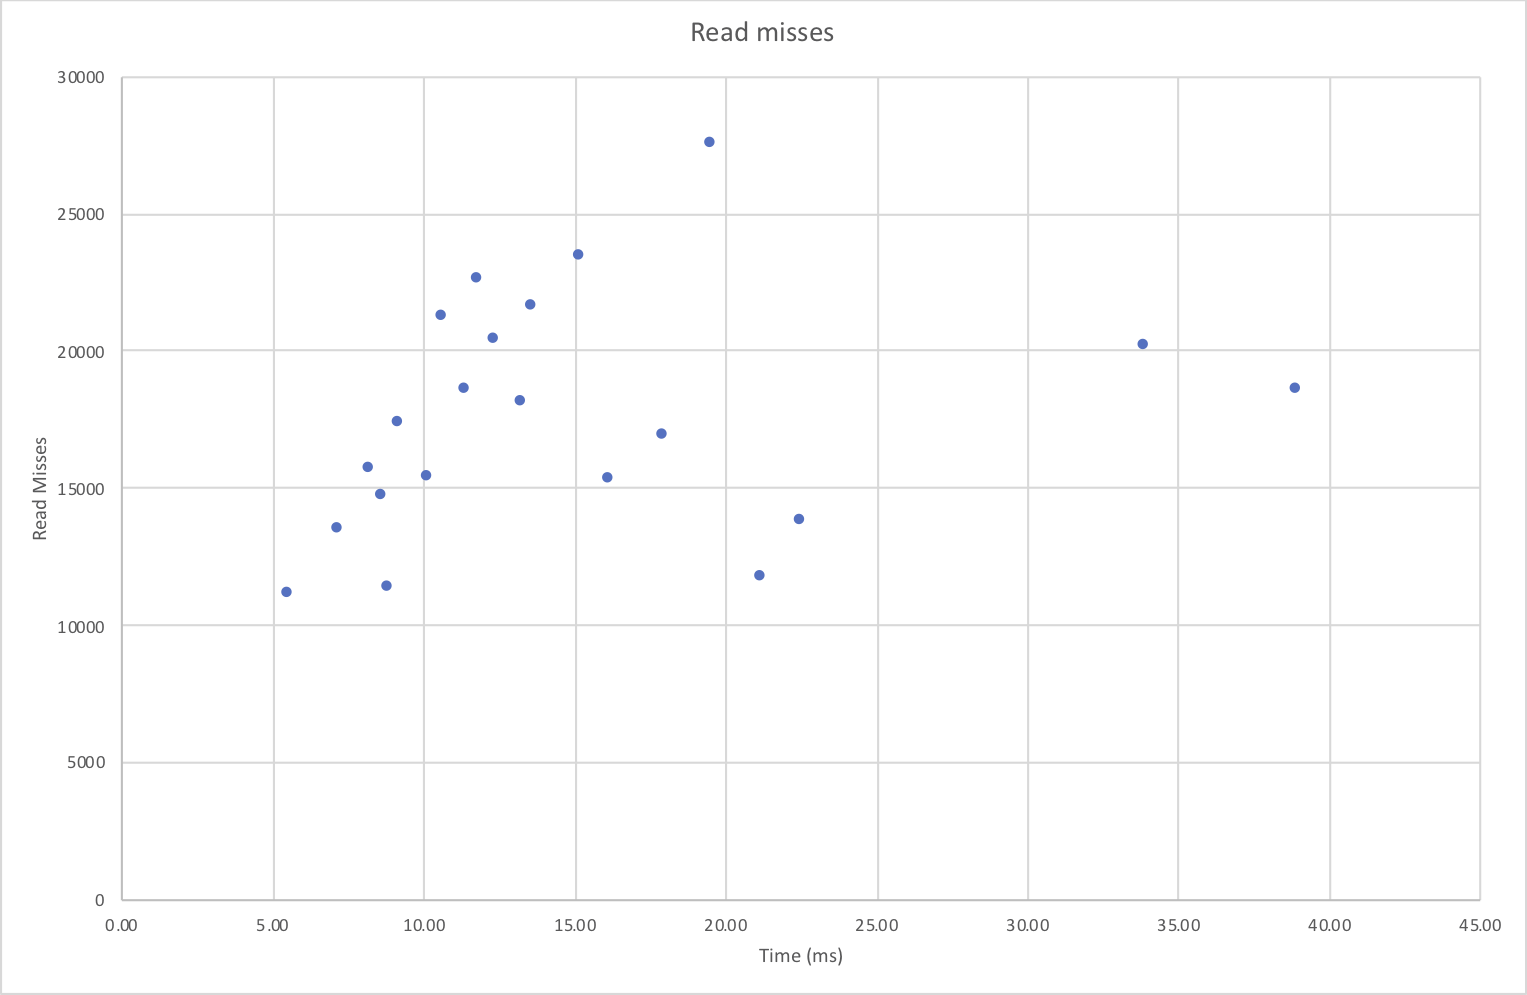
\includegraphics[width=\linewidth]{jetson-readmiss}
  \captionof{figure}{Scatter graph of number of read misses against time taken}
  \label{figure:jetsonreadmiss}
\end{center}

\begin{center}
  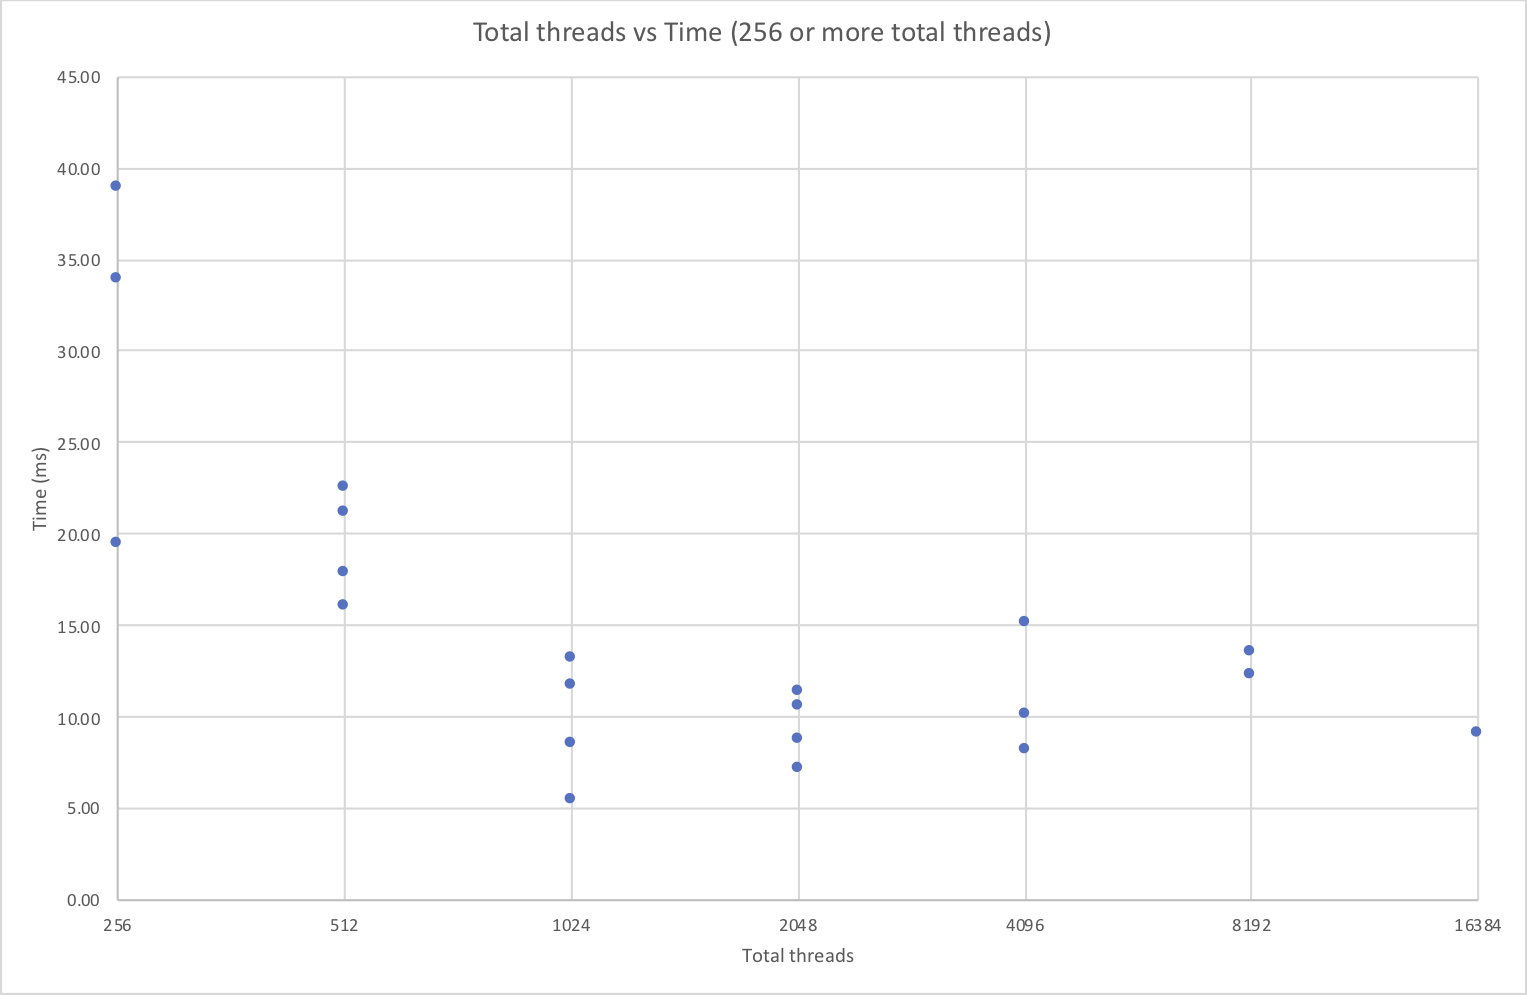
\includegraphics[width=\linewidth]{jetson-saturated}
  \captionof{figure}{Scatter graph of time taken against total threads when $>=256$ total threads are scheduled}
  \label{figure:jetson-saturated}
\end{center}

\subsection{Kernel Performance on XGPC}
The program was run on the Jetson TX2 with blocks-per-grid values between 1 and 80 and threads-per-block values between 1 and 256.

\begin{center}
  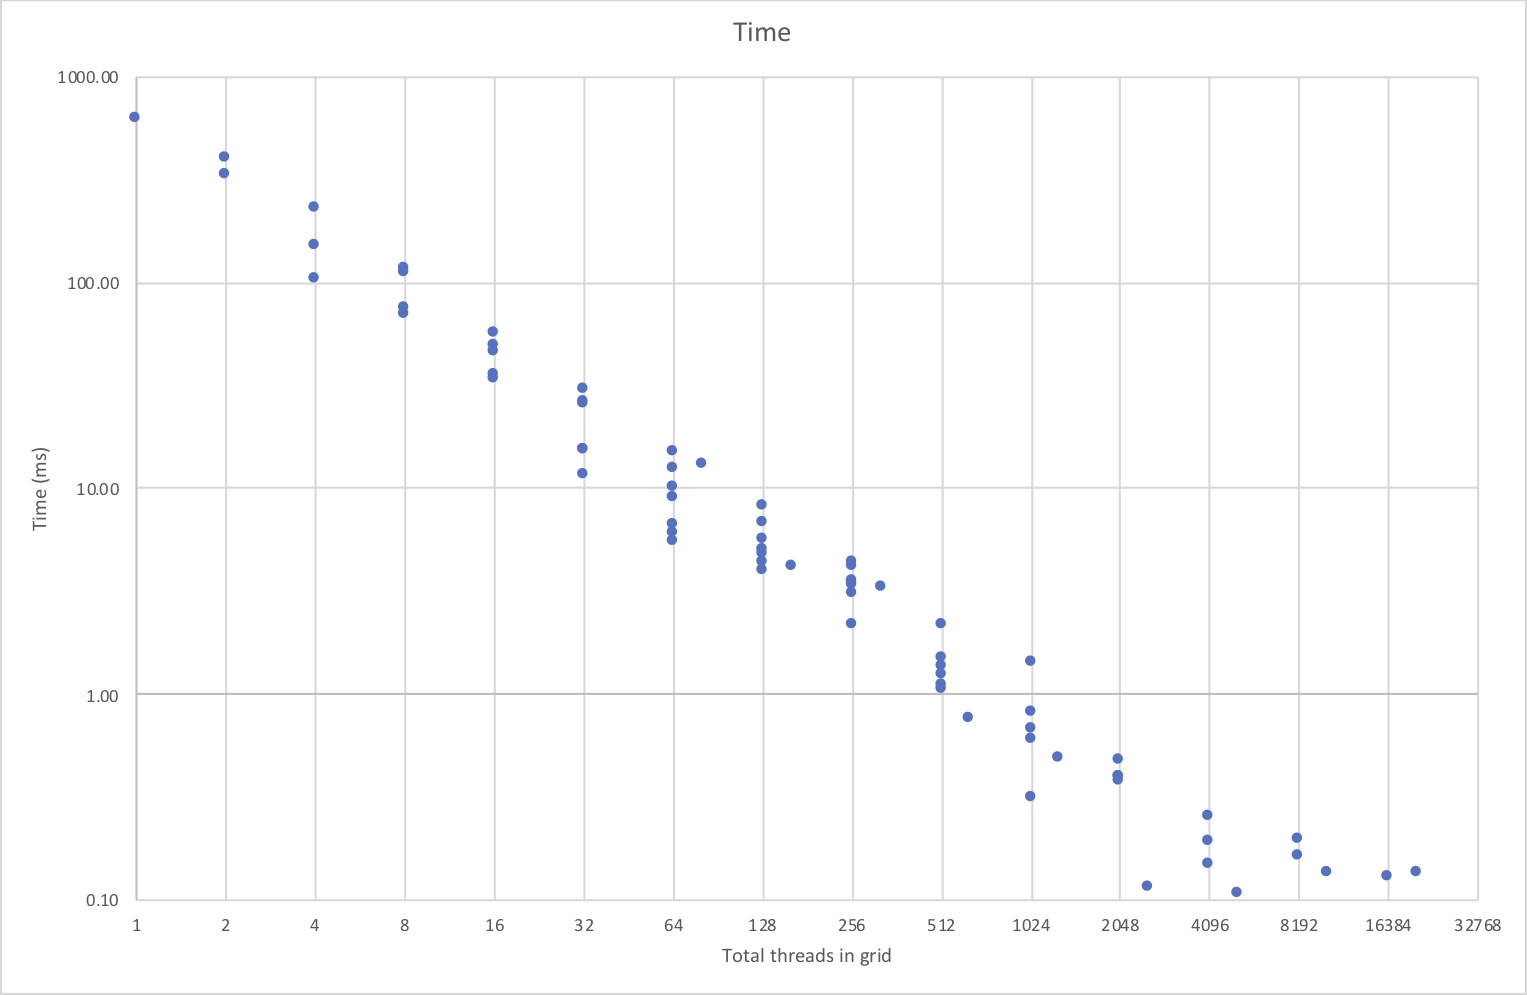
\includegraphics[width=\linewidth]{xgpc-time}
  \captionof{figure}{Scatter graph of time taken on XGPC against total threads in grid}
  \label{figure:xgpctime}
\end{center}

\begin{center}
  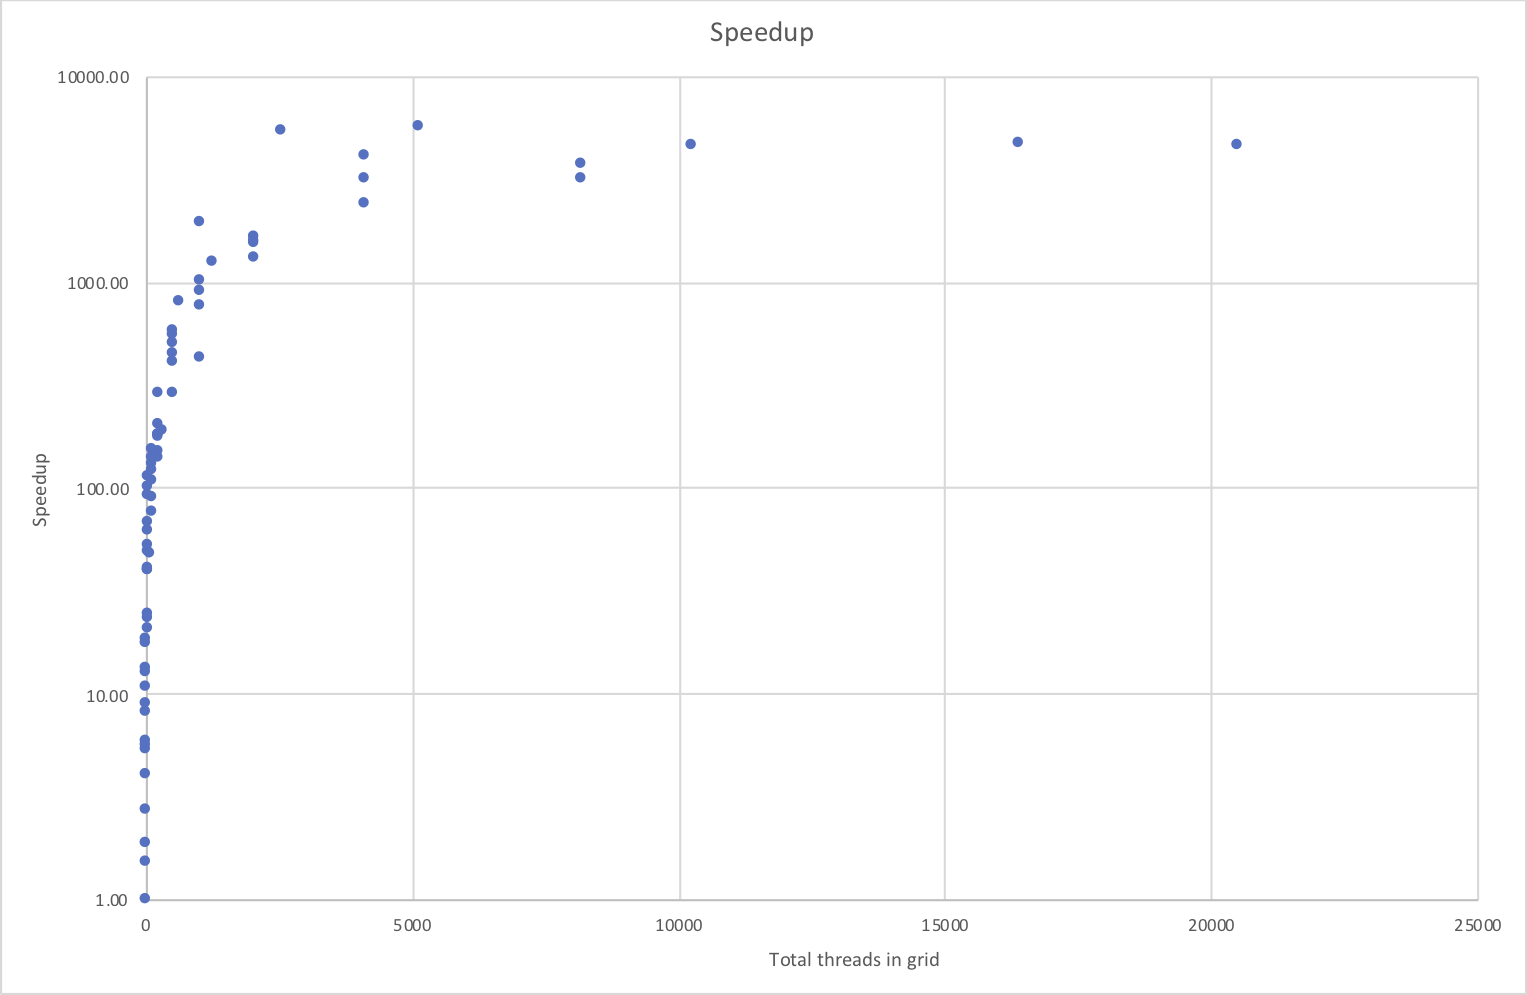
\includegraphics[width=\linewidth]{xgpc-speedup}
  \captionof{figure}{Scatter graph of speedup achieved on XGPC as number of threads increases}
\end{center}

\begin{center}
  \begin{tabular}{r r | r | r}
    No of blocks & No of threads/block & Total threads & time/s \\ \hline
    80 & 64 & 5120 & 0.11 \\
    80 & 128 & 10240 & 0.13 \\
    80 & 256 & 20480 & 0.14 \\
  \end{tabular}
  \captionof{table}{Increasing the total number of threads/block has negligible impact on performance}
  \label{table:xgpcperf}
\end{center}

\subsection{Kernel Stall Dependency}
\begin{center}
  \begin{tabular}{l | r r r}
    Node & stall\_inst\_fetch/\% &	stall\_exec\_dependency/\% &	stall\_memory\_dependency/\% \\ \hline
    Jetson & 10.83 & 26.82 & 49.98 \\
    XGPC & 15.09 & 55.15 & 17.56 \\
  \end{tabular}
  \captionof{table}{Comparison of kernel stall dependency categories according to \texttt{nvprof}}
  \label{table:stall}
\end{center}

\subsection{Discussion}
We observe from the results above that in general, the program becomes faster when the number of total threads increases on both Jetson and XGPC. This trend can be attributed to the following reasons:
\begin{itemize}
  \item Each block can only be executed by a single SM. Therefore, the program performs better when the number of blocks is at least equal to the number of available SMs.
  \item The number of threads per block should be at least equal to the number of CUDA cores on each SM to ensure that all CUDA cores are utilised.
  \item Performance continues to improve even as the number of threads per block exceeds the number of CUDA cores available on each SM. This is because the GPU can hide memory latency when there are extra schedulable warps by executing an alterative warp when the currently active warp is waiting for a memory operation. The large number of registers on the GPU allows it to maintain the execution state of multiple threads at once and thus perform very low cost "context switches". This behaviour is most noticeable on the Jetson TX2 because $49.98\%$ of stalls are due to memory dependency (Table \ref{table:stall}).
\end{itemize}

The experiments on the Jetson TX2 demonstrate the powerful ability of the GPU to hide memory latency. When considering the test cases where there are at least 2 blocks and 256 total threads, we can see that there is little correlation between read misses and execution time (Figure \ref{figure:jetsonreadmiss}). It is more important to ensure that there is a large number of schedulable threads so that the GPU can hide memory latencies effectively (Figure \ref{figure:jetson-saturated}).

Due to the extremely fast memory on the Tesla GPU, tests on the XGPC node were mostly bottlenecked by execution dependencies (Table \ref{table:stall}). Memory access was the cause for only 17.56\% of stalls. As a result, the best speedup was achieved when the program spawned exactly one thread for each CUDA core. Scheduling additional threads actually has a negligible impact on performance (Table \ref{table:stall} and Figure \ref{figure:xgpctime}).

\begin{center}
  \begin{tabular}{l | r r r}
    Node & Serial/$ms$ & Parallel(best)/$ms$ &	Speedup \\ \hline
    Jetson & 1747.5 & 5.51 & 317.19 \\
    XGPC & 618.12 & 0.11 & 5699.89 \\
  \end{tabular}
  \captionof{table}{Comparison of serial and best parallel execution time.}
  \label{table:speedupcomp}
\end{center}

When considering the overall performance on the Jetson and XGPC, we can see that the Tesla GPU in the XGPC is significantly more powerful than the Jetson in both serial and parallel workloads (Table \ref{table:speedupcomp}).

\section{Performance Comparison with OpenMP implementation}

In this section, we shall compare the performance of our CUDA application with an alternative multi-threaded CPU OpenMP implementation.

The OpenMP implementation closely follows the design of the CUDA application. The primary difference is that the kernel code is wrapped in an \mintinline{C}{#pragma omp parallel} block. The storing of the result is protected by a \mintinline{C}{#pragma omp critical} block.

The following tests were executed on a compute cluster node (XGPC6). The OpenMP implementation was executed with 32 threads, matching the number of CPU threads on the machine. The CUDA implementation was executed with 80 blocks per gird and 64 threads per block, following the result of the previous section. Both implementations were run for target values between $2^{30}$ and $2^{48}$.

\begin{center}
  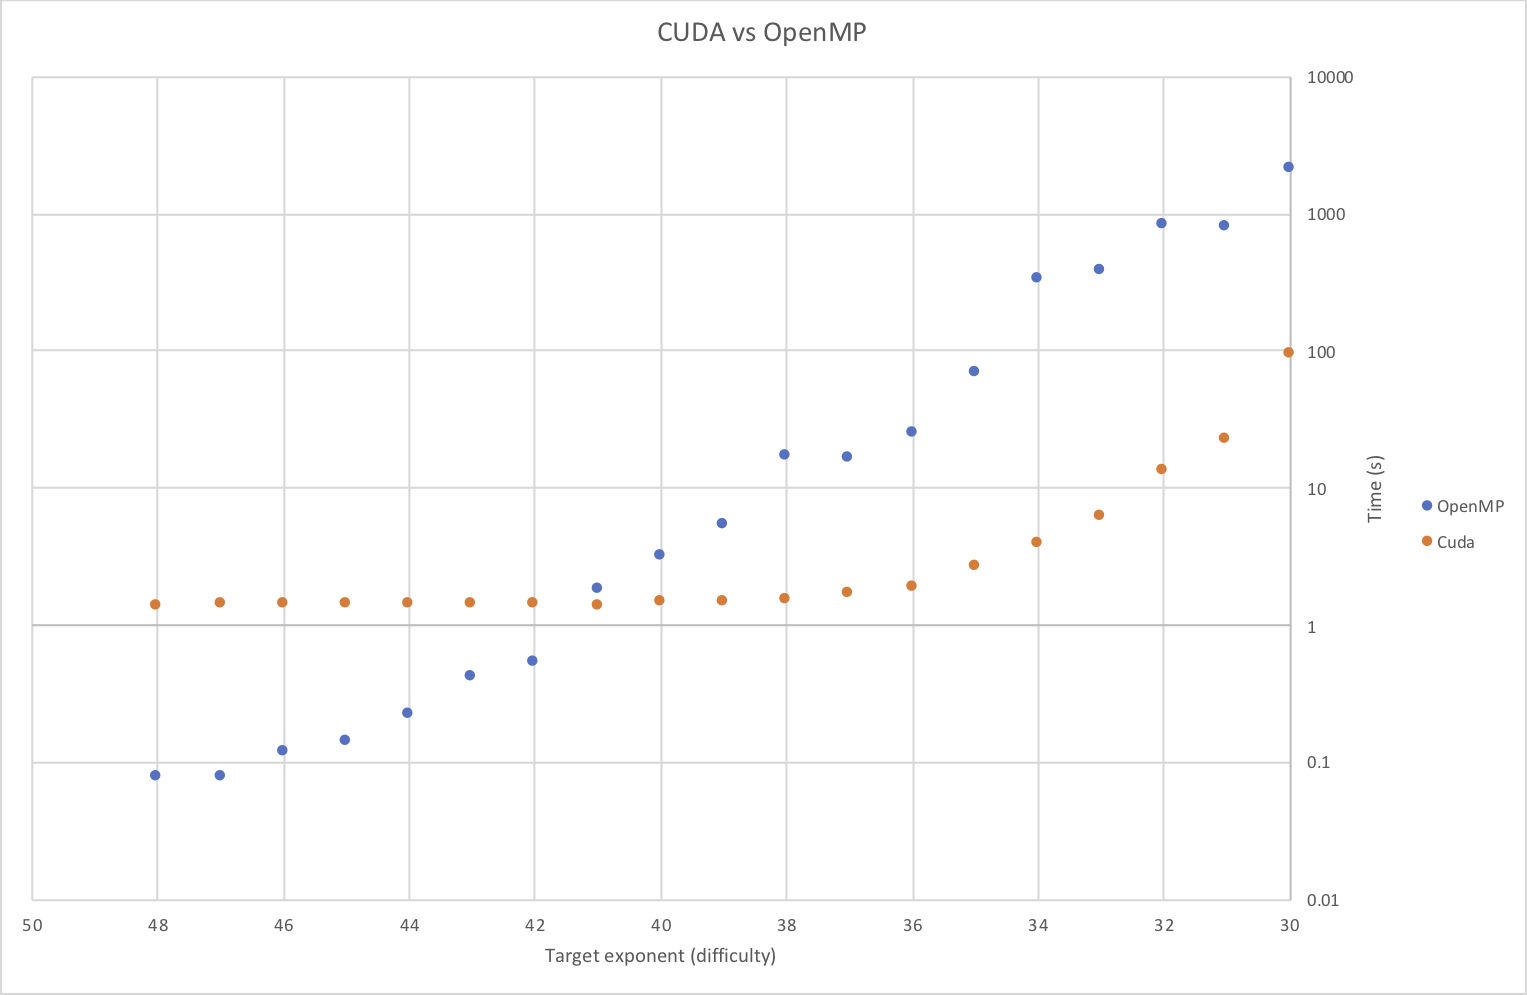
\includegraphics[width=\linewidth]{cuda-vs-openmp}
  \captionof{figure}{Scatter plot of time taken against target exponent of CUDA vs OpenMP implementations}
  \label{figure:cudavsopenmp}
\end{center}

\subsection{Discussion}

Figure \ref{figure:cudavsopenmp} illustrates how data transfer between the host and device can be costly. Under the CUDA implementation, execution time is almost constant for targets between $2^{48}$ and $2^{37}$. This is because the data transfer cost incurred is orders of magnitude greater than the computation cost. We know from the previous section that the kernel itself takes approximately $0.11 ms$, while the total program required $1.41 s$ to complete.

Since the OpenMP implementation did not have to incur this data transfer cost, it was significantly faster when the problem size was small (target was large). However, as the problem size becomes larger, the CUDA implementation took the lead. The data transfer cost was only incurred once regardless of program size, and no data transfers are necessary during the computation itself.

Thus, for larger (easier) target values whose computation time on CPU is shorter than the time taken to copy data to GPU, it is better to use the OpenMP implementation and vice versa.

\newpage
\end{document}
